\chapter{Kondo Breakdown in a Heavy-Fermion Model}
\section{Bilayer extended Hubbard model: Impurity model}
\cite{Mukherjee_2023}
We approach the heavy-fermion problem by starting from a bilayer extended Hubbard model, consisting of two layers (\(f\) and \(c\)). Towards studying this lattice model, we adopt a two-layer impurity problem that hosts a correlated impurity site in each layer (\(S_f\) and \(S_d\)):
\begin{equation}\begin{aligned}
	H_\text{aux} = H_\text{1p} + H_f + H_d + H_{fd}~,
\end{aligned}\end{equation}
where \(H_\text{1p}\) is  the Hamiltonian for the non-interacting itinerant electrons of either layer,
\begin{equation}\begin{aligned}
	H_\text{1p} = -t\sum_{\sigma,\alpha}\sum_{\braket{i,j}}\left(c^\dagger_{i,\sigma,\alpha}c_{j,\sigma,\alpha} + \text{h.c.}\right) - \sum_{i,\sigma,\alpha}\mu_\alpha n_{i,\sigma,\alpha}~,
\end{aligned}\end{equation}
such that \(\alpha\) sums over the two layers \(f\) and \(d\). \(H_f\) and \(H_d\) describe the dynamics of the correlated impurity sites (and their local neighbourhood) in each layer:
\begin{equation}\begin{aligned}
	H_f = -\frac{U_f}{2} (n_{f,\uparrow} - n_{f,\downarrow})^2 + \sum_{Z \in \text{NN}}&\left[-V\sum_{\sigma}\left(c^\dagger_{f,\sigma} c_{Z,\sigma,f} + \text{h.c.}\right) + \frac{J}{2}\sum_{\alpha,\beta}{\bf S}_f \cdot {\boldsymbol{\sigma}}_{\alpha\beta}c^\dagger_{Z,\alpha,f}c_{Z,\beta,f} \right.\\
		 &\left.- \frac{W_f}{2} \left(n_{Z,\uparrow,f} - n_{Z,\downarrow,f}\right)^2\right] ~,\\
	H_d = -\eta_d n_{d} - \frac{U_d}{2}(n_{d,\uparrow} - n_{d,\downarrow})^2 + \sum_{Z \in \text{NN}}&\left[-V\sum_{\sigma}\left(c^\dagger_{d,\sigma} c_{Z,\sigma,d} + \text{h.c.}\right) + \frac{J}{2}\sum_{\alpha,\beta}{\bf S}_d \cdot {\boldsymbol{\sigma}}_{\alpha\beta}c^\dagger_{Z,\alpha,d}c_{Z,\beta,d}\right] ~,
\end{aligned}\end{equation}
where \(c^\dagger_{\nu,\sigma,\alpha}\) can refer to creation operator for either the \(f-\)layer. Finally, \(H_{fd}\) represents the inter-layer hybridisation:
\begin{equation}\begin{aligned}
	H_{fc} = -V_\perp\sum_{\sigma}\left(c^\dagger_{d,\sigma} c_{f,\sigma} + \text{h.c.}\right)~.
\end{aligned}\end{equation}

\section{Tiling Into Bilayer Extended Hubbard Model}
Tiling the impurity model leads to a bilayer extended Hubbard model on the 2D square lattice. In order to tile our auxiliary model to restore translation invariance, we identify the cluster which acts as the ``unit" cell of translation. As discussed in the text surrounding eq.~\ref{clusterHamiltonian}, a good choice for the unit cell is the impurity site and it's surrounding correlated environment. Placing the impurity sites at \(\bm r_d\) in each layer, we get
\begin{equation}\begin{aligned}
	H_\text{clust}(\bm r_d) = H_f(\bm r_d) + H_d(\bm r_d) + H_{fc}(\bm r_d)~.
\end{aligned}\end{equation}
The details of tiling a cluster Hamiltonian were already shown in Sec.~\ref{hamiltonianTile}; the general idea is to use manybody translation operators (details in Sec.~\ref{translationOperators}) to center the cluster Hamiltonian at various sites of the lattice, such that combining all such terms leads to a periodised Hamiltonian. we write down the final result here:
\begin{equation}\begin{aligned}
	H_\text{latt} =& \sum_r T^\dagger(\bm r) H_\text{clust}(\bm r_d) T(\bm r)\\
	=& -\frac{2V}{Z}\sum_{\langle i,j \rangle ,\sigma}\left(c^\dagger_{i,\sigma}c_{j,\sigma} + \text{h.c.}\right) - \sum_i \left[\eta_d n_{i,d} + \frac{U_d}{2}(n_{i,\uparrow,d} - n_{i,\downarrow,d})^2\right] + \frac{2J}{Z}\sum_{\langle i,j \rangle}{\bm S}_{i,d}\cdot{\bm S}_{j,d}\\
				   & -\frac{2V}{Z}\sum_{\langle i,j \rangle ,\sigma}\left(f^\dagger_{i,\sigma}f_{j,\sigma} + \text{h.c.}\right) - \frac{U_f - W_f}{2}\sum_i \left(n_{i,\uparrow,f} - n_{i,\downarrow,f}\right)^2 + \frac{2J}{Z} \sum_{\langle i,j \rangle}{\bm S}_{i,f}\cdot{\bm S}_{j,f}\\
				   & - V_\perp \sum_{i,\sigma}(f^\dagger_{i,\sigma} c_{i,\sigma} + \text{h.c.})
\end{aligned}\end{equation}
Tiling the impurity model therefore leads to a bilayer extended Hubbard model, with effective couplings that depend on the auxiliary model couplings. The value of \(\eta_d\) defines the effective chemical potential of the \(d-\)layer; a non-zero value moves the layer away from half-filling. The \(f-\)layer is pinned at half-filling.


Following Sec.~\ref{tileKspaceGreen}, the retarded \(k-\)space Greens function in either layer can be expressed in terms of  auxiliary model Greens functions:
\begin{equation}\begin{aligned}
	G(\bm k,\sigma,\alpha;\omega) = \sum_\nu C_{\nu,\bm k\alpha}\mathcal{G}(\mathcal{T}_{\nu,\sigma,\alpha}; \omega - \mathcal{E}_\nu(\bm k))
\end{aligned}\end{equation}
where \(\alpha=f,d\) denotes the layer in which the Greens function is being calculated, the modes \(\nu\) indicate the operators which diagonalise the Hamiltonian \(H_\text{1p}\), with energies \(\mathcal{E}_\nu(\bm k)\):
\begin{equation}\begin{aligned}
	H_\text{1p} = -\frac{2V}{Z}\sum_{\langle i,j \rangle ,\sigma}\left(c^\dagger_{i,\sigma}c_{j,\sigma} + \text{h.c.} + f^\dagger_{i,\sigma}f_{j,\sigma} + \text{h.c.}\right) - V_\perp \sum_{i,\sigma}(f^\dagger_{i,\sigma} c_{i,\sigma} + \text{h.c.}) -\sum_i \eta_d n_{i,d}~,
\end{aligned}\end{equation}
and the \(\mathcal{T}-\)matrices are defined in eq.~\ref{tmatrix}:
\begin{equation}\begin{aligned}
	\mathcal{T}_{\nu,\sigma,\alpha} = \left[\left(\sum_{\sigma^\prime}c^\dagger_{\bm \alpha\sigma} + \text{h.c.}\right) + \left(S_{\bm \alpha}^+ + \text{h.c.}\right) + \left(C_{\bm \alpha}^+ + \text{h.c.}\right)\right]c_{\nu,\sigma}~,
\end{aligned}\end{equation}
In order to calculate \(\mathcal{E}_\nu(\bm k)\), we introduce the \(k-\)space modes via a Fourier transform:
\begin{equation}\begin{aligned}
	c^\dagger_{i,\sigma} =\frac{1}{\sqrt N}\sum_{\bm k} e^{-i \bm k \cdot \bm r_i} c^\dagger_{\bm k,\sigma}~,\quad f^\dagger_{i,\sigma} = \frac{1}{\sqrt N}\sum_{\bm k} e^{-i \bm k \cdot \bm r_i} f^\dagger_{\bm k,\sigma}~.
\end{aligned}\end{equation}
In terms of these modes, the \(1-\)particle Hamiltonian decouples in \(k-\)space:
\begin{equation}\begin{aligned}
	H_\text{1p} &= \sum_{\bm k,\sigma}\left[(\epsilon_{\bm k} - \eta_d) (n_{\bm k,\sigma, d} + n_{\bm k,\sigma, f}) - V_\perp(c^\dagger_{\bm k,\sigma}f_{\bm k,\sigma} + \text{h.c.})\right]~.
\end{aligned}\end{equation}
The diagonal modes are given by
\begin{equation}\begin{aligned}
	\nu^\dagger_{\bm k,\sigma,\pm} = C_{\pm,k} c^\dagger_{\bm k,\sigma} + \sqrt{1 - C_{\pm,k}^2}f^\dagger_{\bm k,\sigma}~,
\end{aligned}\end{equation}
the coefficients obtained from diagonalising the matrix
\begin{equation}\begin{aligned}
	H_\text{1p}(\bm k) = \begin{pmatrix} \epsilon_{\bm k}  & -V_\perp\\ -V_\perp & \epsilon_{\bm k} - \eta_d \end{pmatrix}~.
\end{aligned}\end{equation}
The energies are given by \(\mathcal{E}_\pm(\bm k) = \epsilon_k -\eta_d/2 \pm \Delta\), with \(\epsilon_k\) being \(-\frac{4V}{Z}(\cos k_x + \cos k_y)\) for a 2D square lattice and \(\Delta = \sqrt{V_\perp^2 + \eta_d^2/4}\).
Substituting into the expression for the lattice Greens function, we get
\begin{equation}\begin{aligned}
	G(\bm k,d;\omega) =& C_{+, \bm k}\mathcal{G}(\mathcal{T}_{\bm k+,d}, \mathcal{T}^\dagger_{\bm k,d}; \omega - \mathcal{E}_+(\bm k)) + C_{-, \bm k}\mathcal{G}(\mathcal{T}_{\bm k-,d}, \mathcal{T}^\dagger_{\bm k,d}; \omega - \mathcal{E}_-(\bm k))\\
					   &+ C^*_{+, \bm k}\mathcal{G}(\mathcal{T}_{\bm k,d}, \mathcal{T}^\dagger_{\bm k+,d}; \omega - \mathcal{E}_+(\bm k)) + C^*_{-, \bm k}\mathcal{G}(\mathcal{T}_{\bm k,d}, \mathcal{T}^\dagger_{\bm k-,d}; \omega - \mathcal{E}_-(\bm k))	~.
\end{aligned}\end{equation}

Following eq.~\ref{localTiledGreenF}, we can similarly write down an expression the local lattice Greens function for the \(f-\) and \(d-\)electrons. For that, we define the local diagonal modes \(\nu_\pm\) obtained from the local Hamiltonian
\begin{equation}\begin{aligned}
	H_\text{loc} = \begin{pmatrix} 0  & -V_\perp\\ -V_\perp & 0 - \eta_d \end{pmatrix}~,
\end{aligned}\end{equation}
and their associated energies \(\varepsilon_\pm\). Within the impurity model, these local bonding/antibonding modes can be constructed on the impurity sites (\(\nu_\pm\)) or on the neighbouring bath sites, (\(\nu^Z_\pm\)). The local Greens function can be expressed in terms of these modes:
\begin{equation}\begin{aligned}
	G_{dd}(\omega) =& \frac{1}{2}\sum_{\nu}C_{\nu, d} \left[\mathcal{G}(\nu\sigma, d\sigma; \omega - \varepsilon_{\nu}) + \mathcal{G}(d\sigma, \nu\sigma; \omega - \varepsilon_{\nu})\right]\\
								  &+ \frac{1}{2}\sum_{\nu^Z}C_{\nu^Z, Z_d} \left[\mathcal{G}(\mathcal{T}_{Z_d, \sigma}, \mathcal{T}_{\nu^Z,\sigma}; \omega - \varepsilon_{\nu^Z}) + \mathcal{G}(\mathcal{T}_{\nu^Z,\sigma}, \mathcal{T}_{Z_d, \sigma}; \omega - \varepsilon_{\nu^Z})\right]~.
\end{aligned}\end{equation}
The presence of local hybridisation between the \(d-\) and \(f-\) orbitals makes the inter-orbital Greens function important as well. Following eq.~\ref{interorbital}, we have
\begin{equation}\begin{aligned}
	G_{fd}(\omega) =& \frac{1}{2}\sum_{\nu} \left[C_{\nu, f}\mathcal{G}(\nu\sigma, d\sigma; \omega - \varepsilon_{\nu}) + C_{\nu,d}\mathcal{G}(f\sigma, \nu\sigma; \omega - \varepsilon_{\nu})\right]\\
								  &+ \frac{1}{2}\sum_{\nu^Z}\left[C_{\nu^Z, Z_f}\mathcal{G}(\mathcal{T}_{\nu^Z,\sigma}, \mathcal{T}_{Z_d, \sigma}; \omega - \varepsilon_{\nu^Z}) + C_{\nu^Z, Z_d} \mathcal{G}(\mathcal{T}_{Z_f, \sigma}, \mathcal{T}_{\nu^Z,\sigma}; \omega - \varepsilon_{\nu^Z})\right]~.
\end{aligned}\end{equation}
Using these, we can construct the hybridised Greens function associated with the states \(\nu\):
\begin{equation}\begin{aligned}
	G_{\nu_+}(\omega) = C_{+,d}^2 G_{dd}(\omega) + C_{+,f}^2 G_{ff}(\omega) + C_{+,d}C_{+,f}\left[ G_{df}(\omega) + G_{fd}(\omega)\right]~,
\end{aligned}\end{equation}

% TODO
%%%% ACCOUNT FOR F_n in these expressions.

\section{Unitary RG Analysis of The Bilayer Lattice-Embedded ESIAM}
In the limit of large \(U_\alpha\), we carry out a Schrieffer-Wolff transformation and work with the following low-energy Hamiltonian:
\begin{equation}\begin{aligned}
	H_\text{aux} &= \sum_{{\bf k},\sigma,\alpha}\epsilon_{{\bf k},\alpha}n_{{\bf k},\sigma,\alpha} + \sum_\alpha\sum_{Z \in \text{NN}}\left[\frac{1}{2}J_\alpha\sum_{\sigma,\sigma^\prime}{\bf S}_\alpha \cdot {\boldsymbol{\sigma}}_{\alpha\beta}c^\dagger_{Z,\sigma,\alpha}c_{Z,\sigma^\prime,\alpha} - \frac{W_\alpha}{2} \left(n_{Z,\uparrow,\alpha} - n_{Z,\downarrow,\alpha}\right)^2\right] + J{\bf S}_f \cdot {\bf S}_d~.
\end{aligned}\end{equation}
The Kondo coupling and bath interaction acquire \(k-\)dependence:
\begin{equation}\begin{aligned}
	J({\bf k}, {\bf q}) &= \frac{J}{2}\left[\cos({\bf k}_x - {\bf q}_x) + \cos({\bf k}_y - {\bf q}_y)\right]~,\\
	W({\bf k}, {\bf q}, {\bf k}^\prime, {\bf q}^\prime) &= \frac{W}{2}\left[\cos({\bf k}_x - {\bf q}_x + {\bf k}^\prime_x - {\bf q}^\prime_x) + \cos({\bf k}_y - {\bf q}_y + {\bf k}^\prime_y - {\bf q}^\prime_y)\right]~.
\end{aligned}\end{equation}
The particle-hole transformed state \(\bar{\bf q}\) associated with \({\bf q}\) is defined as \(\bar {\bf q} = {\bf q} + \left(\pi, \pi\right)\) if \({\bf q}\) is in the first or third quadrant and \({\bf q} + \left(\pi, -\pi\right)\) is in the second or fourth quadrant.

In order to study the low-energy physics of the impurity model, we iteratively integrate out high-energy degrees of freedom using the unitary RG method. Let the momentum states being decoupled from the two layers be \(\ket{{\bf q},\sigma,f}\) and \(\ket{{\bf q},\sigma,d}\) if they are above the Fermi energy (unoccupied in the low-energy configuration) and \(\ket{\bar{\bf q},\sigma,f}\) and \(\ket{\bar{\bf q},\sigma,d}\) if they are below the Fermi energy (occupied in the low-energy configuration)
For every shell of conduction bath states of width \(\Delta D\) integrated out, the Hamiltonian couplings renormalise by folding in the effects of virtual excitations to these states. We already have the renormalisation group equations for the couplings \(J_\alpha\) in the case of \(J=0\):
\begin{equation}\begin{aligned}
	\frac{\Delta J_f({\bf k}_1, {\bf k}_2)}{\Delta D} = -\int_{UV} d{\bf q} ~\rho({\bf q}) \left[J_f({\bf k}_1, {\bf q})J_f({\bf q}, {\bf k}_2) + 4J_f({\bf q}, \bar {\bf q})W_f({\bf k}_1, {\bf q}, \bar {\bf q}, {\bf k}_2)\right] G_f^{(0)}({\bf q})~,
\end{aligned}\end{equation}
where \({\bf q}\) sums over the UV states being integrated out, \(\rho({\bf q})\) is the density of states for the momentum states being integrated out and \(G_f^{(0)}\) is the propagator for the excited intermediate state (for \(J=0\)):
\begin{equation}\begin{aligned}
	G_f^{(0)}({\bf q}) = \frac{1}{\omega - |\epsilon_f({\bf q})| / 2 + J_f({\bf q}) / 4 + W_f({\bf q}) / 2}~.
\end{aligned}\end{equation}
An identical equations holds for \(\Delta J_d\), with al \(f-\)quantities replaced with \(d-\)quantities. Switching on \(J\) modifies the excitation energy in the propagator:
\begin{equation}\begin{aligned}
	G_f({\bf q}) = \frac{1}{1/G_f^{(0)} - J \vec{S}_f\cdot\vec{S}_d}~.
\end{aligned}\end{equation}
This expression can be simplified by noting that the operator in the denominator has only two eigenvalues, \(-3/4\) in the singlet sector and \(1/4\) in the triplet sector. Defining the projectors \(\mathcal{P}_0\) and \(\mathcal{P}_1\) for the two sectors, we have
\begin{equation}\begin{aligned}
	\vec{S}_f\cdot\vec{S}_d = \frac{-3}{4}\mathcal{P}_0 + \frac{1}{4}\mathcal{P}_1, \quad \mathcal{P}_0 + \mathcal{P}_1 = \mathbb{I}~.
\end{aligned}\end{equation}
Using these relations, we can write
\begin{equation}\begin{aligned}
	G_f({\bf q}) &= \frac{1}{1/G_f^{(0)} + 3J/4}\mathcal{P}_0 + \frac{1}{1/G_f^{(0)} - J/4}\mathcal{P}_1 \\
		&= \left(\frac{1/4}{1/G_f^{(0)} + 3J/4} + \frac{3/4}{1/G_f^{(0)} - J/4}\right)\mathbb{I} + \left(\frac{1}{1/G_f^{(0)} + 3J/4} + \frac{1}{1/G_f^{(0)} - J/4}\right)\vec{S}_f\cdot\vec{S}_d~.
\end{aligned}\end{equation}
Noting that only the first operator renormalises the Kondo interaction, we get the following modified RG equation for the Kondo coupling \(J_\alpha\):
\begin{equation}\begin{aligned}
	\frac{\Delta J_\alpha}{\Delta D} = \int_{UV} d{\bf q} ~\rho({\bf q}) \left[J_\alpha({\bf k}_1, {\bf q})J_\alpha({\bf q}, {\bf k}_2) + J_\alpha({\bf q}, \bar {\bf q})W_\alpha({\bf k}_1, {\bf q}, \bar {\bf q}, {\bf k}_2)\right]\left(\frac{1}{4}\frac{1}{1/G_\alpha^{(0)}({\bf q}) + 3J/4}\right.\\
																																																										   \left. + \frac{3}{4}\frac{1}{1/G_\alpha^{(0)}({\bf q}) - J/4}\right)~,
\end{aligned}\end{equation}

We now turn to the renormalisation of \(J\), arising from hybridisation of \(f-\) and \(d-\)layers. In order to capture coherent scattering processes between the two layers, we project onto the following rotated basis of excited states:
\begin{equation}\begin{aligned}
	\ket{H}_\pm &= \frac{1}{\sqrt{2}}\left(\ket{H({\bf q})}_f \pm \ket{H({\bf q})}_d\right)~,\\
	\mathcal{P({\bf q})}_H &= \ket{H}_+\bra{H}_+ + \ket{H}_-\bra{H}_-~,
\end{aligned}\end{equation}
where \(\ket{H({\bf q})}_\alpha\) is the state obtained upon exciting both states in the layer \(\alpha\): \(\ket{H(q)}_\alpha = c^\dagger_{{\bf q},\alpha}c_{\bar {\bf q},\alpha}\ket{L}_f\ket{L}_d\), and \(\mathcal{P({\bf q})}_H\) projects onto this rotated excited basis. We focus on the spin-flip component \(J S_f^+ S_d^-\) of the Hamiltonian. There are two kinds of processes that renormalise this coupling. We first consider one that involves a spin-flip of the \(d-\)layer followed by a spin-flip of the \(f-\)layer:
\begin{equation}\begin{aligned}\label{rgEqtn1}
	\Delta H = \frac{1}{N^2}\sum_{{\bf q} \in \text{UV}}\braket{L | \frac{1}{2}J_f(\bar{\bf q},{\bf q}) S_f^+ c^\dagger_{{\bf q-}_\downarrow,f}c_{{\bf q+}\uparrow,f} \mathcal{P({\bf q})}_H G \mathcal{P({\bf q})}_H\frac{1}{2}J_d({\bf q},\bar{\bf q})S_d^- c^\dagger_{{\bf q}\uparrow,d}c_{\bar {\bf q}\downarrow,d} | L }~,
\end{aligned}\end{equation}
where \(\ket{L} = \ket{L}_f \ket{L}_d\) is the initial configuration for both layers. \(G\) is the propagator for the excited state:
\begin{equation}\begin{aligned}
	G = \frac{1}{\omega - H_D}~,
\end{aligned}\end{equation}
where \(H_D\) is the diagonal part of the Hamiltonian corresponding to the excited(intermediate) state. The diagonal part consists of the kinetic energy and the Ising part of the Kondo interaction:
\begin{equation}\begin{aligned}
	H_D = \sum_{{\bf q,\sigma}\in{\bf q}_\pm, \alpha}\epsilon_\alpha({\bf q})\tau_{{\bf q},\sigma} + \frac{1}{2}\sum_\alpha J_\alpha S_\alpha^z \sum_{{\bf q},\sigma}\sigma n_{{\bf q},\sigma,\alpha} + J \vec{S}_f \cdot \vec{S}_d~.
\end{aligned}\end{equation}
Calculating the matrix elements of the propagator in the rotated basis gives
\begin{equation}\begin{aligned}\label{PGP}
	\mathcal{P({\bf q})}_H G \mathcal{P({\bf q})}_H = \frac{1}{2}\left(G_f + G_d\right)\left(\ket{H}_+\bra{H}_+ + \ket{H}_-\bra{H}_-\right) + \frac{1}{2}\left(G_f - G_d\right)\left(\ket{H}_+\bra{H}_- + \ket{H}_-\bra{H}_+\right)~,
\end{aligned}\end{equation}
where
\begin{equation}\begin{aligned}
	G_\alpha({\bf q}) = \frac{1}{\omega - \frac{1}{2}\left[\epsilon_\alpha({\bf q}) - \epsilon_\alpha(\bar{\bf q})\right] + \frac{1}{2}J_\alpha({\bf q}) + W_\alpha({\bf q}) - \frac{1}{4}J}~.
\end{aligned}\end{equation}

In eq.~\ref{rgEqtn1}, since the first process is an excitation into a \(d-\)state and the second process is a de-excitation from an \(f-\)state, the expression can be simplified into
\begin{equation}\begin{aligned}\label{rgEqtn2}
	\braket{L | S_f^+ c^\dagger_{{\bf q-}_\downarrow,f}c_{{\bf q+}\uparrow,f} \mathcal{P({\bf q})}_H G \mathcal{P({\bf q})}_H S_d^- c^\dagger_{{\bf q+}\uparrow,d}c_{{\bf q-}\downarrow,d} | L } &= S_f^+ S_d^- \braket{H_f | \mathcal{P({\bf q})}_H G \mathcal{P({\bf q})}_H | H_d} \\
																																																 &= \frac{1}{2}\left(G_f + G_d\right) S_f^+ S_d^-~.
\end{aligned}\end{equation}
The net Hamiltonian renormalisation is finally a sum over the contribution from each mode:
\begin{equation}\begin{aligned}
	\Delta H = \frac{1}{8N^2} \sum_{{\bf q} \in \text{UV}}J_f(\bar{\bf q},{\bf q}) J_d({\bf q},\bar{\bf q})\left(G_f({\bf q}) + G_d({\bf q})\right) S_f^+ S_d^-~.
\end{aligned}\end{equation}
Converting the sums to integrals (assuming a density of states \(\rho({\bf q})\)) gives the final expression
\begin{equation}\begin{aligned}
	\frac{\Delta H}{\Delta D} = \frac{1}{8N} S_f^+ S_d^-\int_{UV} d{\bf q} ~\rho({\bf q}) J_f(\bar{\bf q},{\bf q}) J_d({\bf q},\bar{\bf q})\left(G_f({\bf q}) + G_d({\bf q})\right)~.
\end{aligned}\end{equation}

The time-reversed of this process can be obtained simply by exchanging the \(d-\)interaction with the \(f-\)interaction. Since the renormalisation itself is symmetric, the contribution is equal to what we obtained here. The total renormalisation in the coupling for the term \(S_f^+ S_d^-\) is therefore
\begin{equation}\begin{aligned}
	\frac{\Delta J}{\Delta D} &= \frac{1}{2} \int_{UV} d{\bf q} ~\rho({\bf q}) J_f(\bar{\bf q},{\bf q}) J_d({\bf q},\bar{\bf q})\left(G_f({\bf q}) + G_d({\bf q})\right) \\
							  &= \frac{1}{2}\int_{UV} d{\bf q} ~\rho({\bf q}) \left[\frac{J_f(\bar{\bf q},{\bf q}) J_d({\bf q},\bar{\bf q})}{\omega - \frac{1}{2}\bar\epsilon_f({\bf q}) + \frac{1}{2}J_f({\bf q}) + W_f({\bf q}) - \frac{1}{4}J} + \frac{J_f(\bar{\bf q},{\bf q}) J_d({\bf q},\bar{\bf q})}{\omega - \frac{1}{2}\bar\epsilon_d({\bf q}) + \frac{1}{2}J_d({\bf q}) + W_d({\bf q}) - \frac{1}{4}J}\right]~,
\end{aligned}\end{equation}
where \(\bar\epsilon_\alpha({\bf q}) = \epsilon_f({\bf q}) - \epsilon_f(\bar{\bf q})\) is the total excitation energy for the pair of states \({\bf q},\bar{\bf q}\).

Since the bath interaction doesn't renormalise, it's functional form remains unchanged and can be substituted into the RG equations. In fact, we can write the expressions in a compact matrix form for efficient computation:
\begin{equation}\begin{aligned}
	\frac{\Delta J_\alpha}{\Delta D} = -J_\alpha \mathcal{G}_\alpha J_\alpha^\dagger - 4\mathcal{W}_\alpha\text{Tr}\left[\mathcal{G}^\prime_\alpha\right]~,
\end{aligned}\end{equation}
where all objects are matrices. \(J_\alpha\) is the Kondo coupling matrix. \(\mathcal{G}_\alpha\) is a diagonal matrix with matrix elements 
\begin{equation}\begin{aligned}
\mathcal{G}_\alpha[q, q] = \begin{cases}
	\rho(q) \left(\frac{1}{8}\frac{1}{1/G_\alpha^{(0)}({\bf q}) + \mu/2 + 3J/4} + \frac{3}{8}\frac{1}{1/G_\alpha^{(0)}({\bf q}) + \mu/2 - J/4}\right),~{\bf q}\in\text{PS}~,\\
\rho(q) \left(\frac{1}{8}\frac{1}{1/G_\alpha^{(0)}({\bf q}) - \mu/2 + 3J/4} + \frac{3}{8}\frac{1}{1/G_\alpha^{(0)}({\bf q}) - \mu/2 - J/4}\right),~{\bf q}\in\text{HS}~~,
\end{cases}
\end{aligned}\end{equation}
if \(q\) is in the UV subspace and zero otherwise. \(\mathcal{W}_\alpha\) is the bath interaction matrix whose matrix elements are given by \(\mathcal{W}_\alpha[k, k^\prime] = \frac{W}{2}\left[\cos(k_x - k^\prime_x) + \cos(k_y - k^\prime_y)\right]\). Finally, \(\mathcal{G}^\prime_\alpha\) is another diagonal matrix whole matrix elements are defined as \(\mathcal{G}^\prime_\alpha[q,q] = \mathcal{G}[q, q] J_\alpha[q,\bar q]\).

The RG equation for the inter-layer coupling \(J\) can be written as
\begin{equation}\begin{aligned}
	\frac{\Delta J}{\Delta D} &= \frac{1}{2} {\bf J} \cdot \mathcal{\bf G}~,
\end{aligned}\end{equation}
where \({\bf J}\) and \(\mathcal{\bf G}\) are vectors defined by the elements \({\bf J}[q] = J_f(\bar{\bf q},{\bf q}) J_d({\bf q},\bar{\bf q})\) and 
\begin{equation}\begin{aligned}
	\mathcal{\bf G}[q] = \rho({\bf q}) \left[\frac{1}{\omega - \frac{1}{2}\bar\epsilon_f({\bf q}) + \frac{1}{2}J_f({\bf q}) + W_f({\bf q}) - \frac{1}{4}J} + \frac{1}{\omega - \frac{1}{2}\bar\epsilon_d({\bf q}) + \frac{1}{2}J_d({\bf q}) + W_d({\bf q}) - \frac{1}{4}J}\right]~.
\end{aligned}\end{equation}

\section{Renormalisation Group Flows of Kondo Couplings: RG Phase Diagram}
\begin{figure}[!t]
	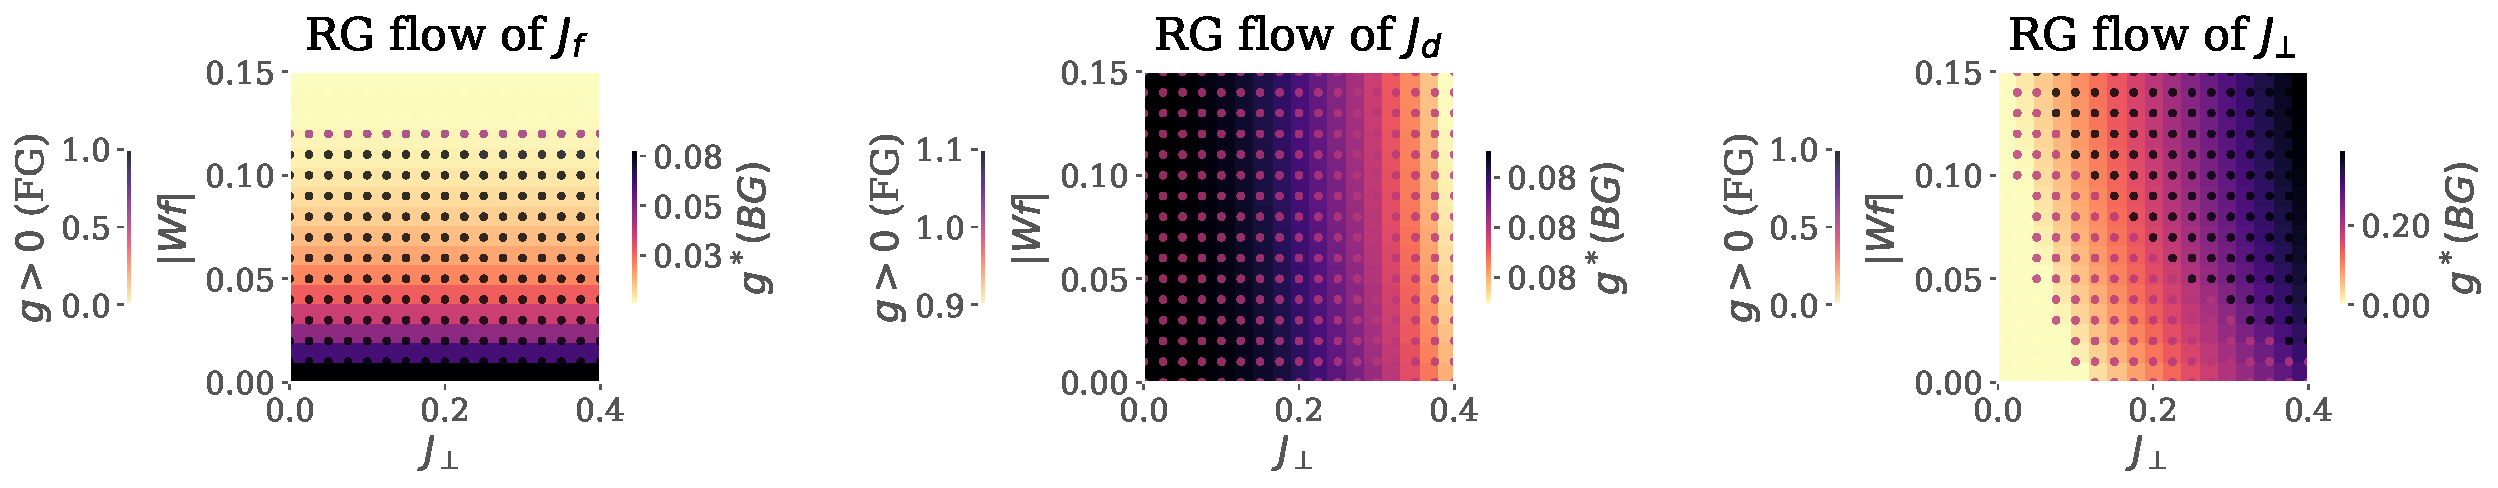
\includegraphics[width=\textwidth]{PD_33.pdf}
	\caption{RG phase diagrams for various Kondo couplings: \(f-\)layer (left), \(d-\)layer (middle) and inter-layer (right). For each plot, the background color (quantified by the right colorbar) tracks the fixed point value of the coupling as a function of the inter-layer couplings \(J_\perp\) and the \(f-\)layer bath interaction \(|W_f|\). The marker color complements this by tracking whether the coupling is relevant, intermediate-coupling or irrelevant in the RG sense, by taking the values 1, \(1/2\) or 0 respectively.}
	\label{couplingRG}
\end{figure}
We first analyse the model by obtaining unitary RG flows of three kinds of Kondo couplings. Fig.~\ref{couplingRG} shows the fixed point values of the couplings under renormalisation to a low-energy theory. We view these values as a function of the \(f-\)layer bath interaction \(W_f\) and inter-layer Kondo coupling \(J_\perp\). In each panel, the right (left) colorbar quantifies the background (marker) color of the plot. The background displays the fixed point value of each coupling whereas the marker color tracks whether the couplings is relevant (1), intermediate coupling (0.5) or irrelevant (0). 

The Kondo coupling \(J_d\) (middle panel) of the \(d-\)layer remains relevant for the entirety of the chosen parameter regime. The Kondo coupling \(J_f\) (left panel) of the \(f-\)layer becomes RG-irrelevant for larger values of \(|W_f|\); this leads to an in-plane Mott transition of the kind observed in our earlier work, where the local Fermi liquid excitations of the \(f-\)impurity give way to a pseudogapped non-Fermi liquid Mott metal phase which ultimately destabilises into a local moment phase. The RG flow of \(J_f\) does not appear to be significantly affected by the variation of \(J_\perp\). Concomitant with the irrelevance of \(J_f\) under increasing \(|W_f|\), the inter-plane coupling \(J_\perp\) (right panel) becomes RG-relevant, as seen from the darkening markers as we go to higher \(|W_f|\). 

These simulations motivate an RG-based phase diagram with the following regimes: (i) weak \(J_\perp\), weak \(|W_f|\): decoupled metallic layers, each layer participating in transport independently, (ii) strong \(J_\perp\), strong \(|W_f|\): Kondo insulator regime, where the local moments of the \(f-\)layer hybridise with the itinerant electrons of the \(d-\)layer to form a band insulator with the chemical potential situated in the hybridisation gap, and (iii) weak \(J_\perp\), strong \(|W_f|\): the so-called RKKY regime, where the \(f-\)layer forms local moments which decouple from the \(d-\)layer and are then free to order magnetically, and (iv) strong \(J_\perp\), weak \(|W_f|\): this is similar to the Kondo insulator regime, except here the \(f-\)electrons remain itinerant and it is they who hybridise with the \(d-\)electrons to again form two bands separated by a hybridisation gap.

\section{Results at half-filling}
\begin{figure}[!h]
	\centering
	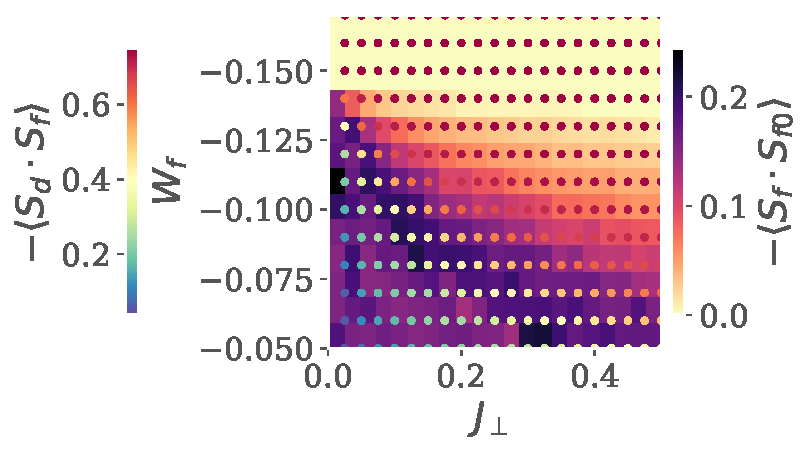
\includegraphics[width=0.4\textwidth]{locCorr_33_1299.pdf}
	\caption{Left: Real-space spin correlations for the auxiliary model. Background colour (right colourbar) represents that between the \(f-\)impurity and its nearest-neighbour sites, while the marker colour (left colourbar) represents that between the \(f-\)impurity and the \(d-\)impurity. While the former shrinks as \(J_\perp\) or \(|W_f|\) is increased, the latter grows. This marks a transfer of entanglement from intra-plane channel into inter-plane channel. Right: }
\end{figure}

\begin{figure}[!h]
	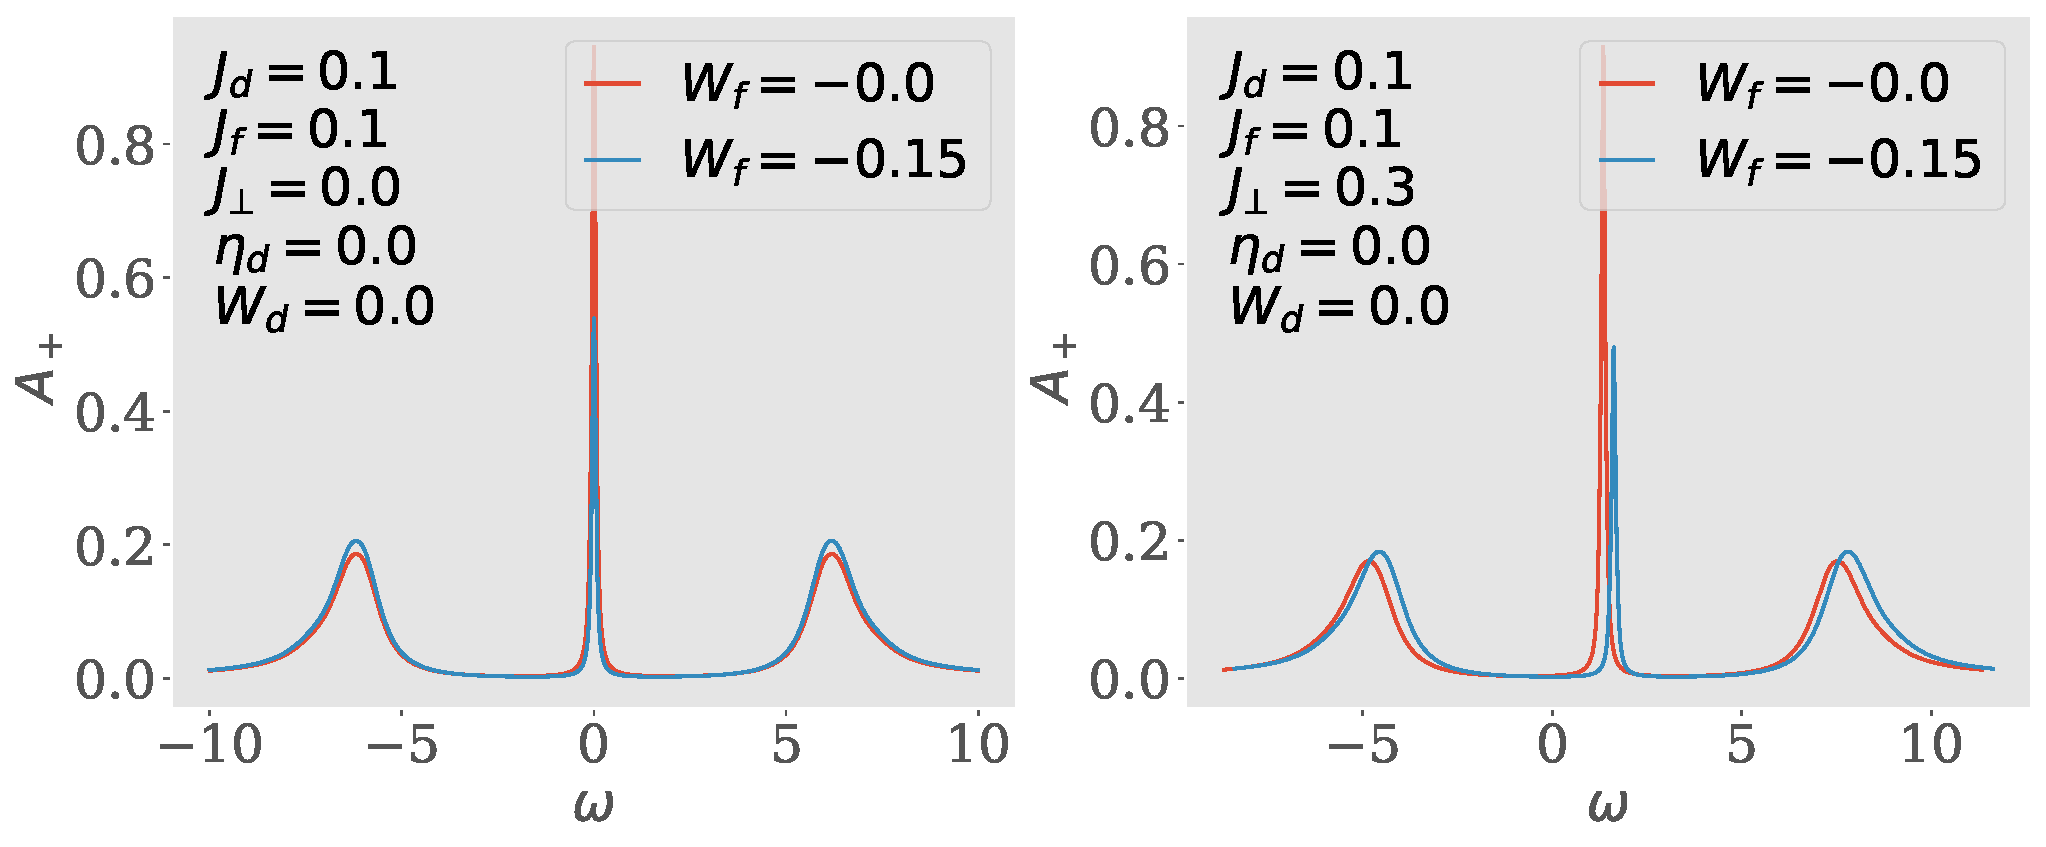
\includegraphics[width=0.49\textwidth]{specFunc_node_+_33_1555.pdf}
	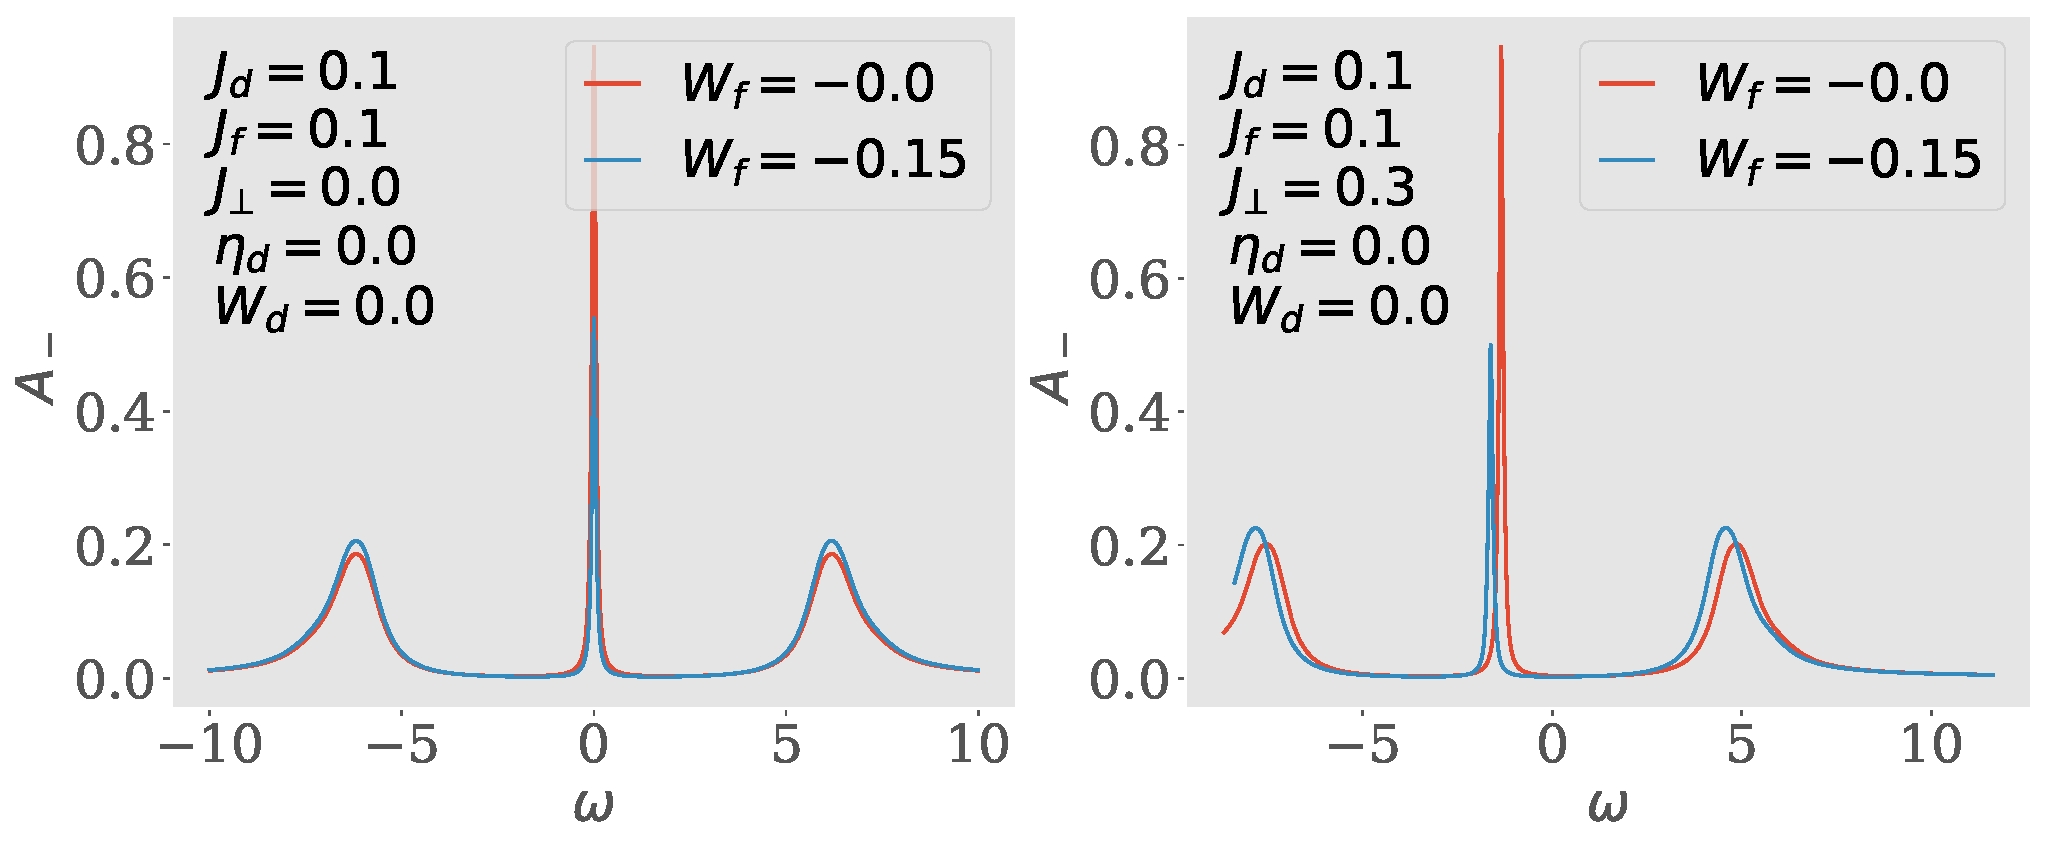
\includegraphics[width=0.49\textwidth]{specFunc_node_-_33_1555.pdf}
		\caption{Spectral functions of the tiled model, for excitations in the bonding (two on the left) and antibonding (two on the right) basis, defined by the Greens function \(G_{k,\pm} = G(k_d \pm k_f; \omega)\). There is no hybridisation for \(J_\perp=0\) (first and third plots), and the only effect of \(W_f\) is to shrink the height of the central resonance. Introducing a non-zero \(J_\perp\) splits the central resonance into an upper band (second from left) and a lower band (first from right). This leads to a Kondo insulator, where \(\omega=0\) resides inside the hybridisation gap.
		}
\end{figure}

\begin{figure}[!h]
	\centering
	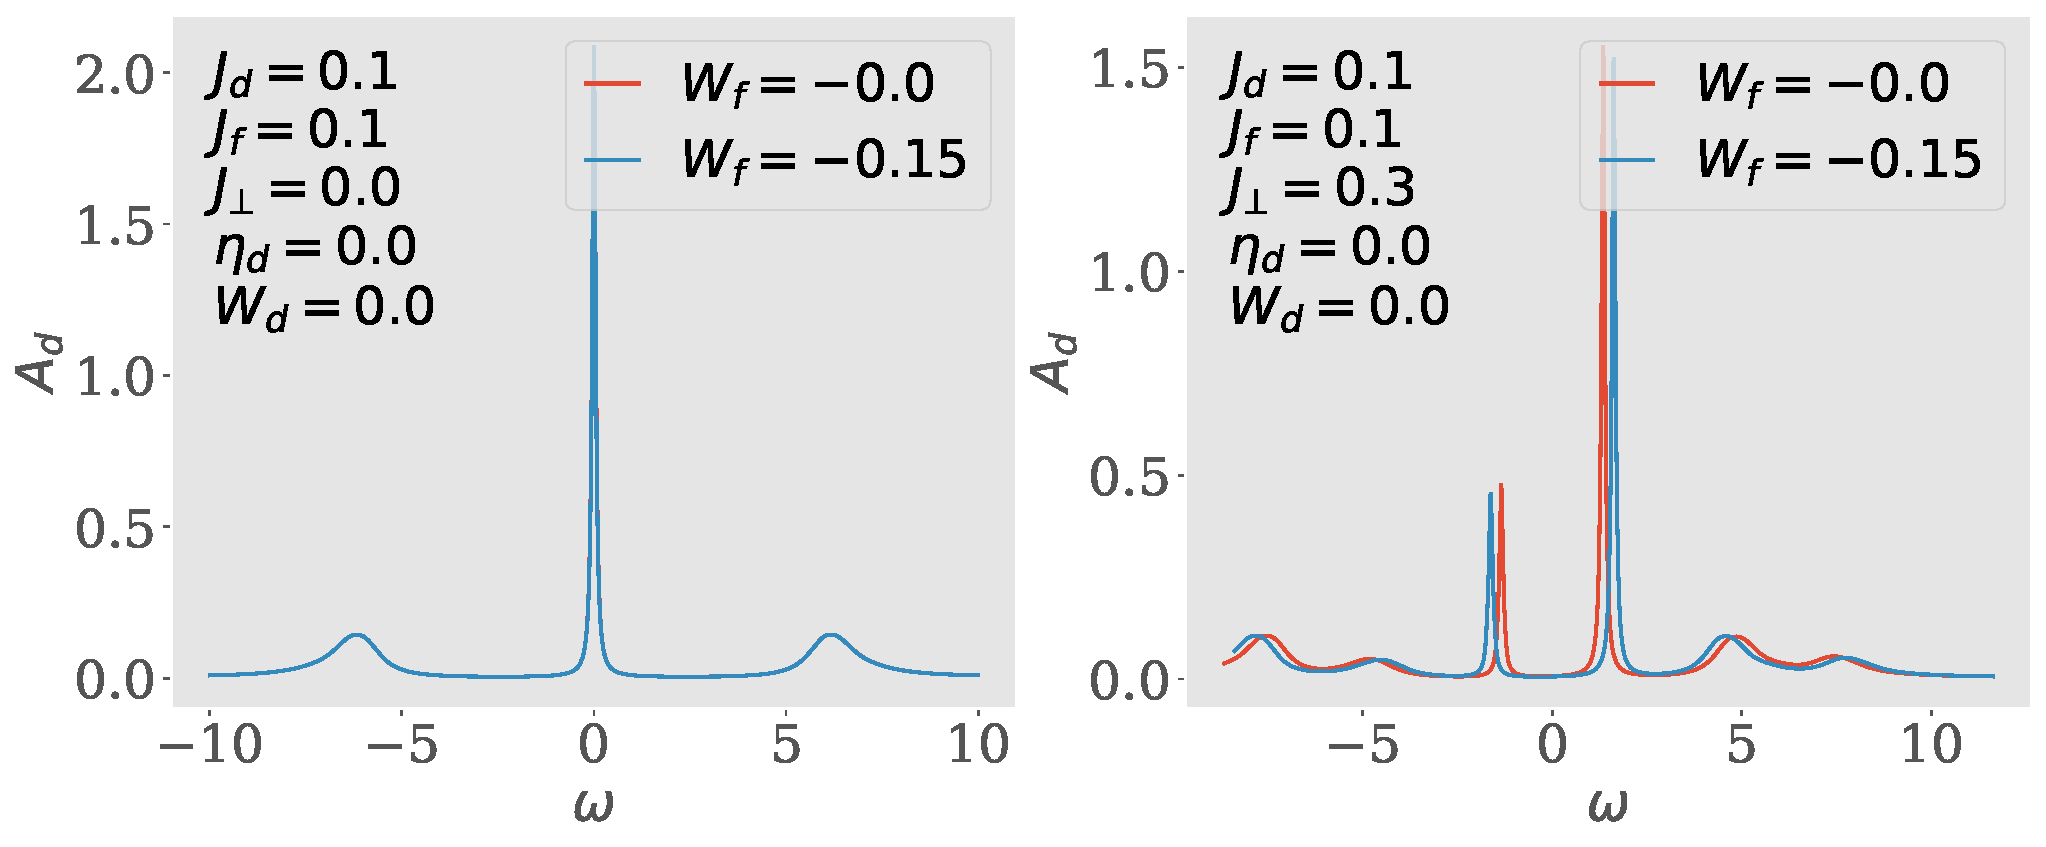
\includegraphics[width=0.49\textwidth]{specFunc_node_d_33_1555.pdf}
	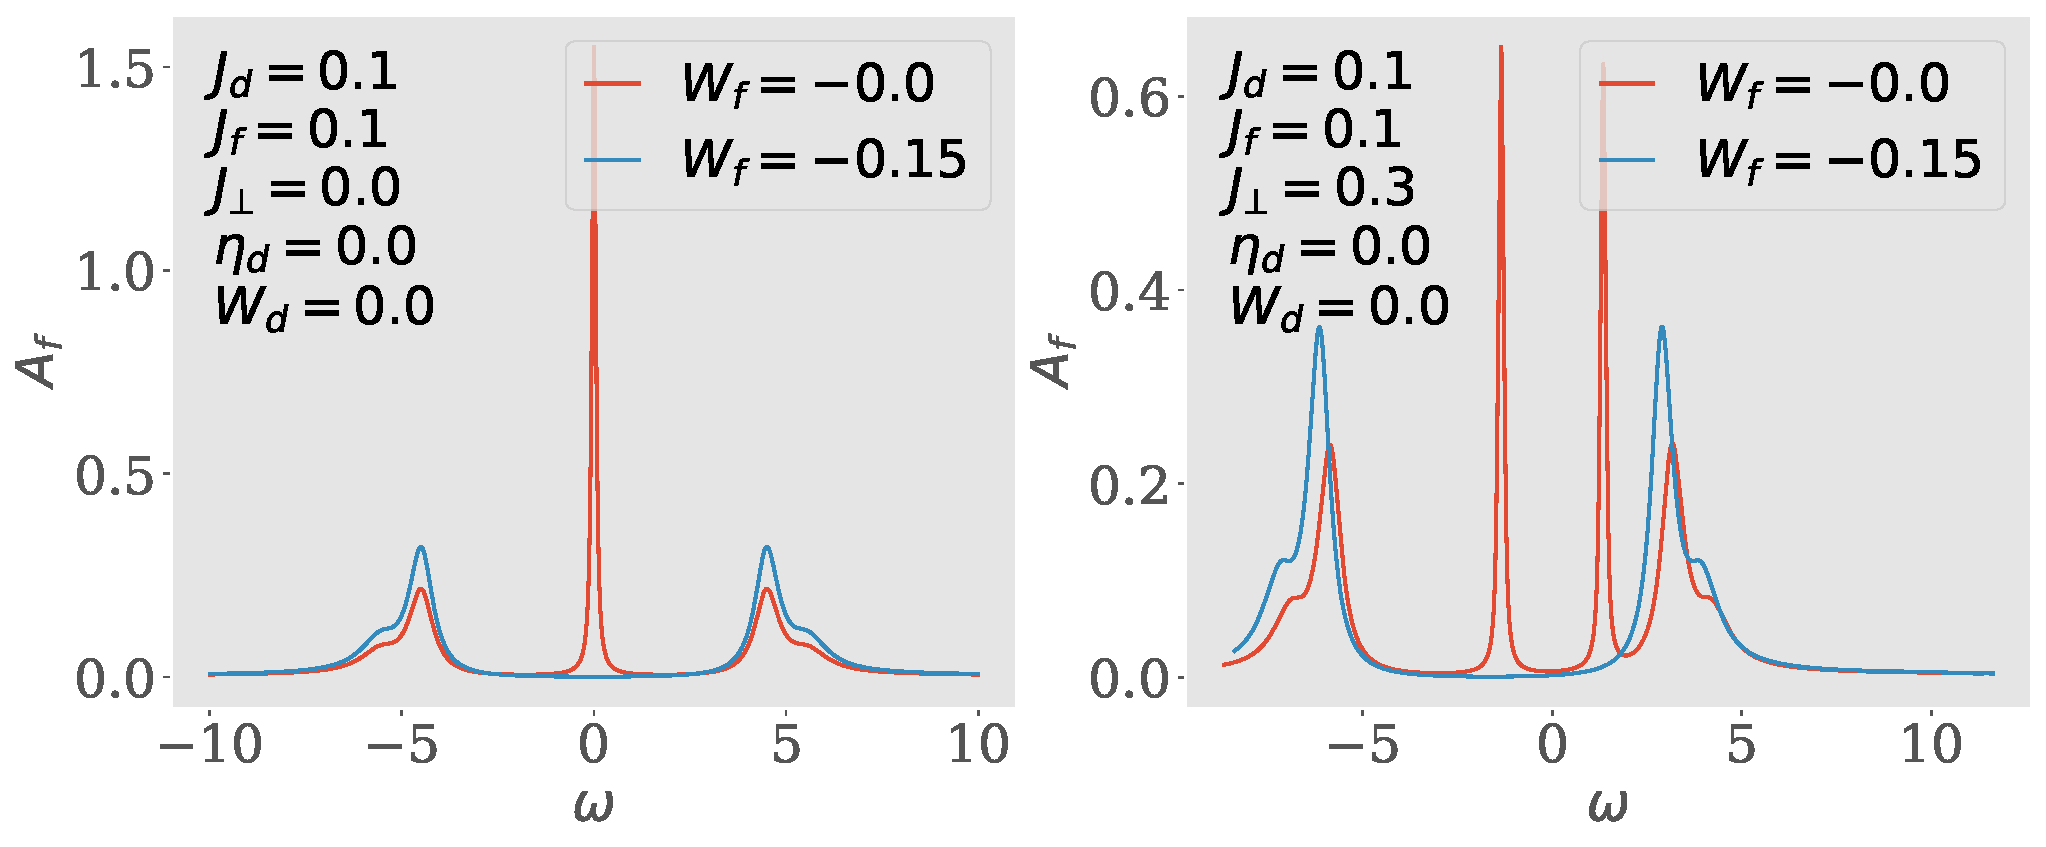
\includegraphics[width=0.49\textwidth]{specFunc_node_f_33_1555.pdf}
	\caption{Spectral functions \(A_d\) and \(A_f\) of the auxiliary model, for excitations in the \(d-\) and \(f-\)layers respectively. Both show a central Kondo resonance for \(J_\perp=0\) which splits into two bands upon adding a non-zero \(J_\perp\). Increasing \(|W_f|\) to large values gaps out the local Fermi liquid excitations of \(A_f\).
	}
\end{figure}
